\documentclass[final]{beamer}
% http://tex.stackexchange.com/questions/56205/wrapfigure-beamer-style
\usepackage{color}
\usepackage{transparent}
%\usepackage{enumitem}
%\usepackage{cutwin}
%\usetheme{RJH}
\usetheme{irishep}
%\usetheme{Bergen}
\usepackage[orientation=portrait,size=a0,scale=1.4,debug]{beamerposter}
\usepackage[absolute,overlay]{textpos}
\setlength{\TPHorizModule}{1cm}
\setlength{\TPVertModule}{1cm}
\beamertemplatenavigationsymbolsempty
% RGB (145,201,219), #91C9DB
%\definecolor{mybluelabel}{RGB}{145,201,219}
% RGB (48,174,228), #30AEE4
\definecolor{mybluelabel}{RGB}{48,174,228}

% Turn off list indentation
%\setlist[itemize]{leftmargin=*}

\begin{document}
\begin{frame}{} 

\begin{textblock}{80.0}(2,2)
\begin{center}
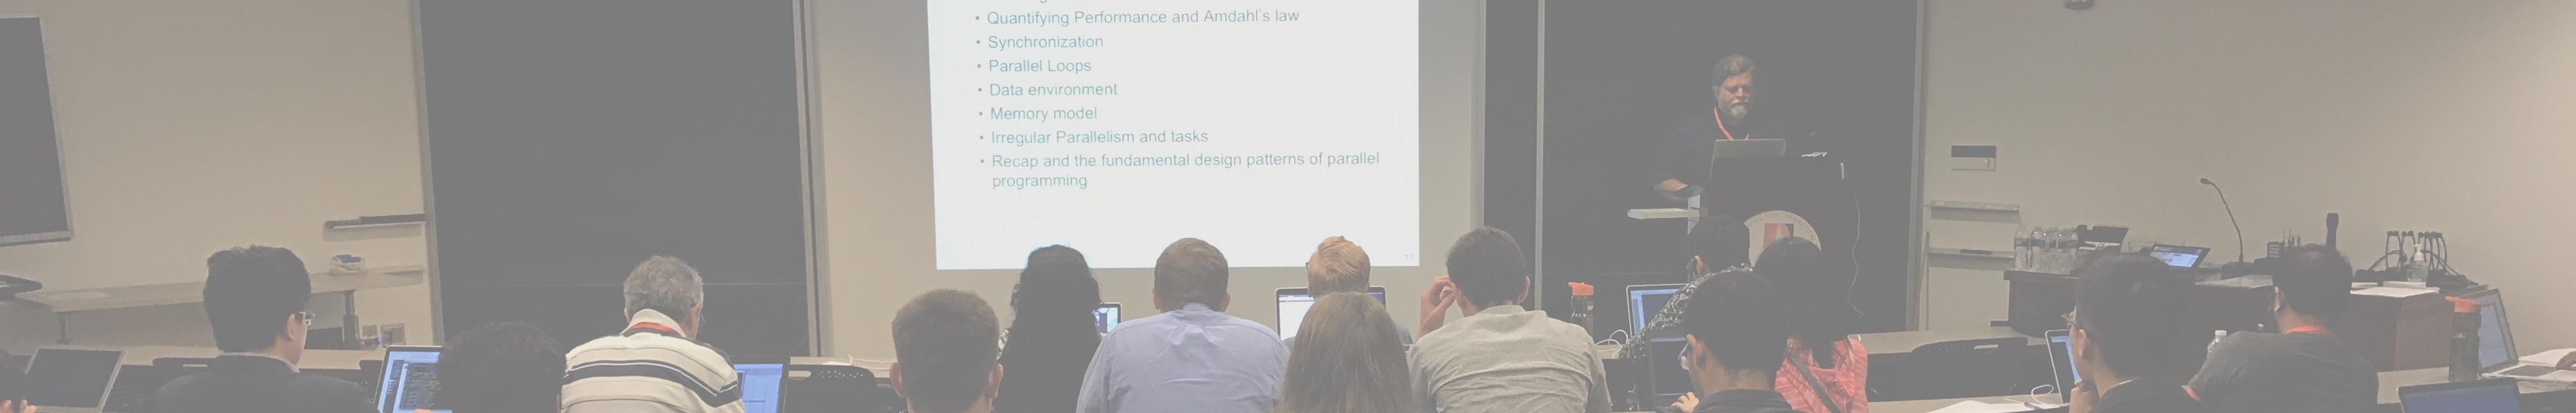
\includegraphics[width=1.00\textwidth]{images/codashep2017-mattson-class-IMG_6311-slice.JPG}
\end{center}
\end{textblock}

\begin{textblock}{84.0}(0,3)
\begin{center}
\begin{Huge}
%\color{white}{
\textbf{
Framework for Integrated Research Software Training \\
~~in High Energy Physics (FIRST-HEP)
}
%}
\end{Huge}
\end{center}
\end{textblock}

\begin{textblock}{84.0}(2,8.8)
\begin{center}
\begin{Large}
\textbf{
PIs: Peter Elmer (Princeton Univ.), Ian Cosden (Princeton Univ.)\\ 
, Sudhir Malik (Univ. of Puerto Rico at Mayaguez)
}
\end{Large}
\end{center}
\end{textblock}


\begin{textblock}{80.0}(2,15)
\begin{block}{Science Driver: Discoveries beyond the Standard Model of Particle Physics}

\begin{textblock}{16.0}(2,17)
\begin{figure}[H]
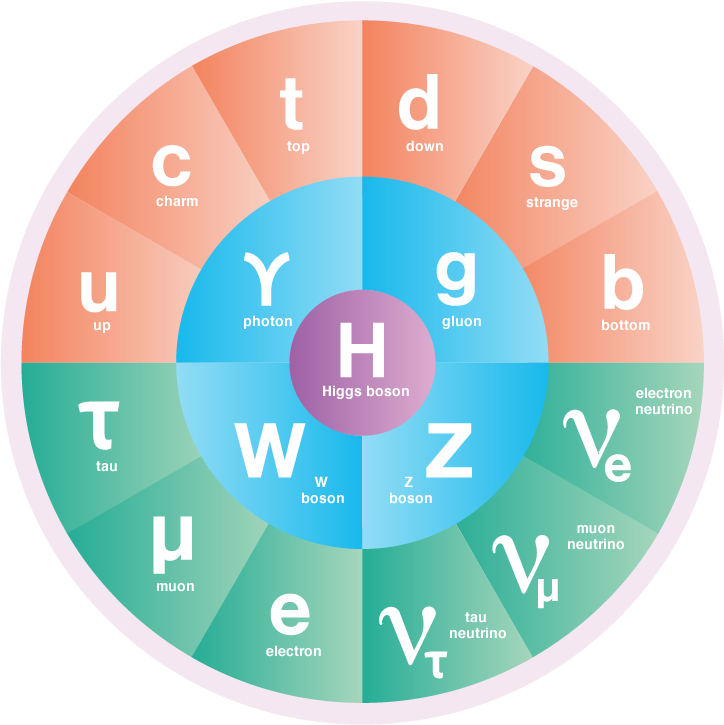
\includegraphics[width=0.87\textwidth]{images/standard_model_ai.png}
\end{figure}
\end{textblock}

\begin{textblock}{50.0}(20,18)
{\it From ``Building for Discovery - Strategic Plan for U.S. Particle Physics in the Global \\
Context'' - Report of the Particle Physics Project Prioritization Panel (P5):}

\begin{center}
\begin{enumerate}
\item Use the Higgs boson as a new tool for discovery
\item Pursue the physics associated with neutrino mass
\item Identify the new physics of dark matter
\item Understand cosmic acceleration: dark matter and inflation
\item Explore the unknown: new particles, interactions, and physical principles
\end{enumerate}
\end{center}
\end{textblock}

\begin{textblock}{16.0}(64,16)
\begin{figure}[H]
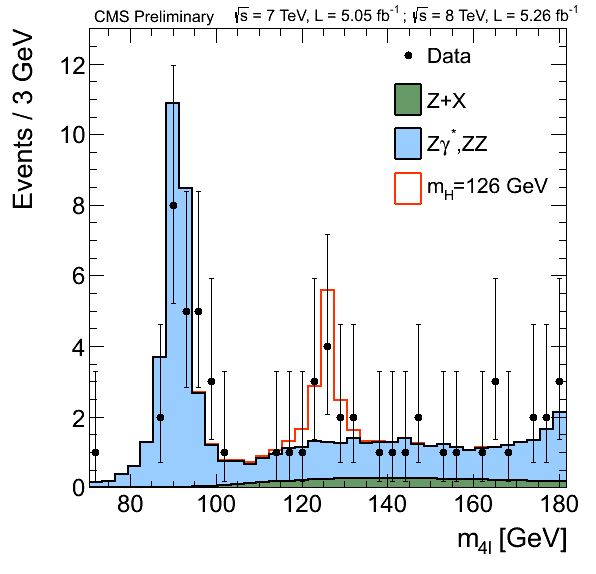
\includegraphics[width=0.95\textwidth]{images/Fig4-ZZMass_7Plus8TeV_70-180_3GeV.png}
\end{figure}
\end{textblock}

\end{block}
\end{textblock}

%%%%%%%%%%%%%%%%%%%%%%%%%%%%%%%%%%%%%%%%%%%%%%%%%%%%%%%%%%%%%%%%%%%%%%%%%%%%%%


\begin{textblock}{38.0}(2,32)
\begin{block}{The FIRST-HEP Project}
\begin{textblock}{38.0}(2,34)
Goals achieved:
\begin{itemize}
\item Build an international community around training for particle, nuclear and astroparticle physics and a common model for a multi-step/tiered evolution of training (See Training Pyramid)
\item Develop a Carpentries-style curriculum relevant for that community and widely-used by the international community
\item With the community execute both introductory training activities in the US and internationally and an advanced US summer school (CoDaS-HEP), with specific individuals progressing through multiple training activities. Clear examples of individuals eventually contributing to widely used research software (via the IRIS-HEP software institute, e.g. Scikit-HEP, mkFit, or via experiments such as CMS or LHCb)
\item 1016 people trained to date (with 175 instructors engaged), a mix of many in-person and virtual training events (COVID-driven/limited) → students become instructors and mentors
\item Current focus is scalability and sustainability of these activities
\end{itemize}
\end{textblock}
\end{block}
\end{textblock}



\begin{textblock}{38.0}(44,32)
\begin{block}{A Larger Vision for Training}
\begin{textblock}{38.0}(44,34)
\begin{figure}[tbph]
\centering
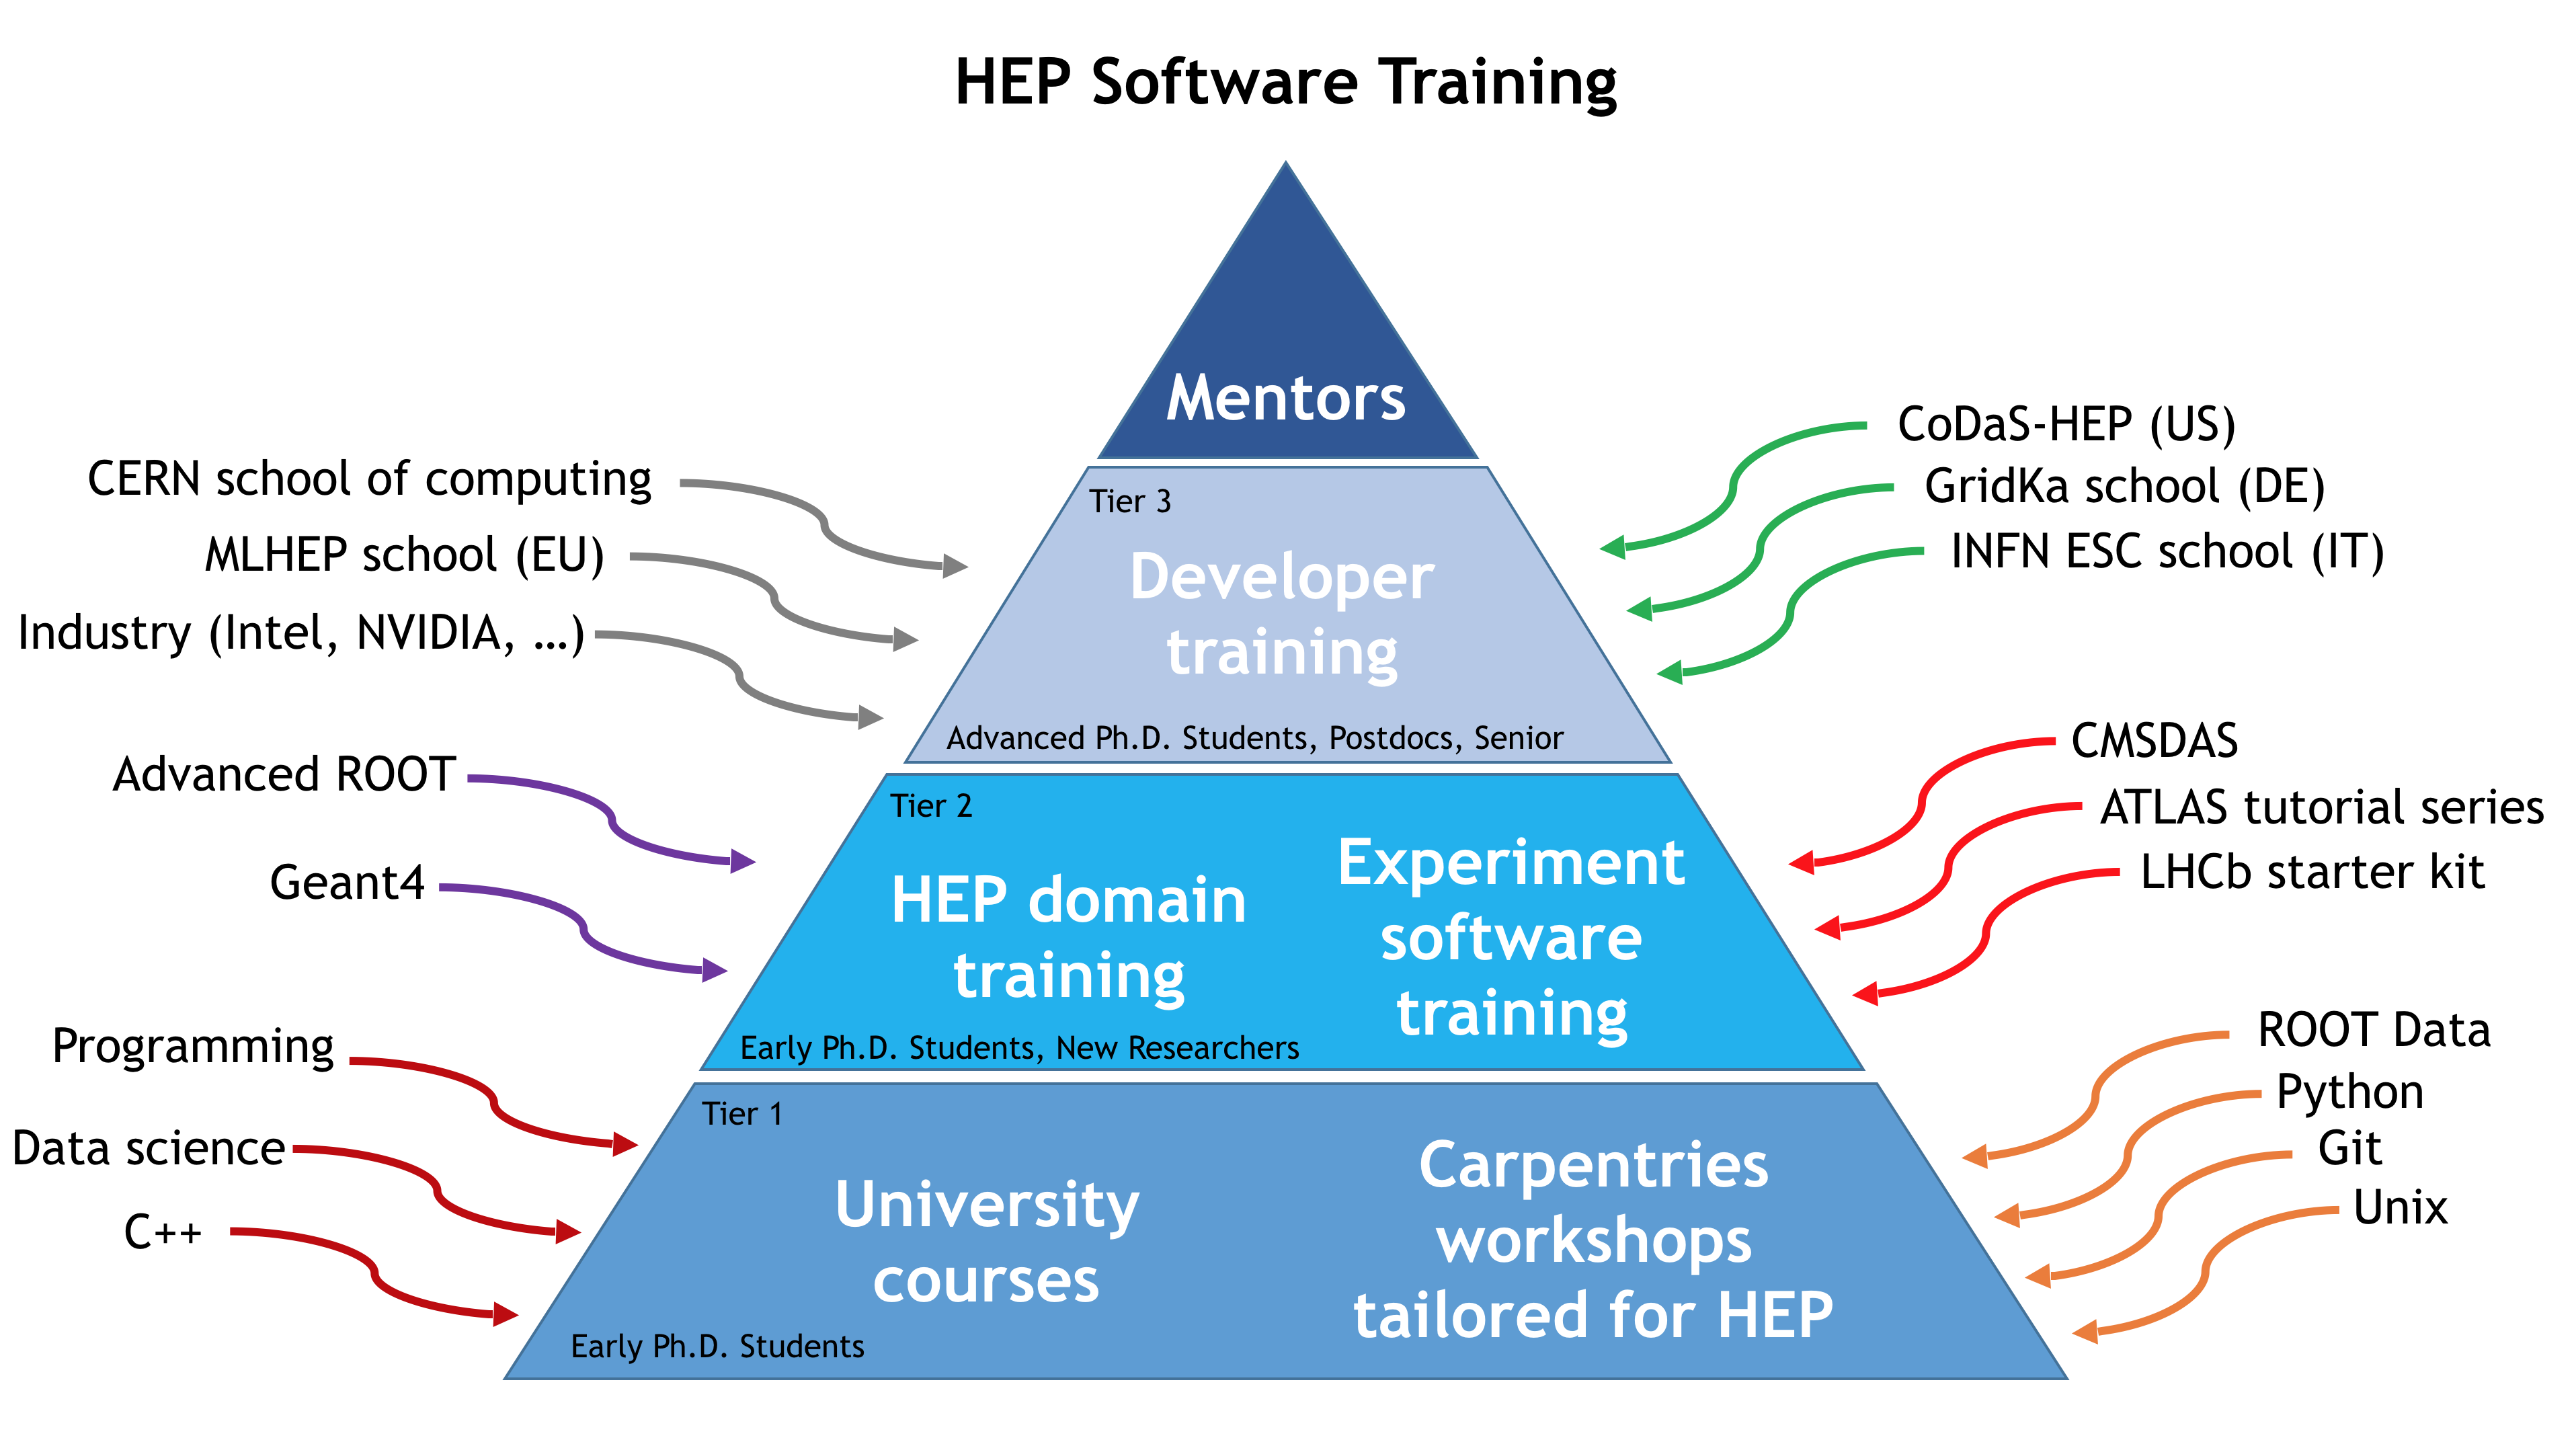
\includegraphics[width=1.00\textwidth]{images/Training-Pyramid.png}
\end{figure}
Training participants can evolve from basic software skills through more advanced training via offerings from the training framework.
\end{textblock}
\end{block}
\end{textblock}

\begin{textblock}{19.0}(44,61)
\begin{block}{Software Carpentries Aug. 2021}
\begin{textblock}{19.0}(44,63)
\begin{figure}[tbph]
\centering
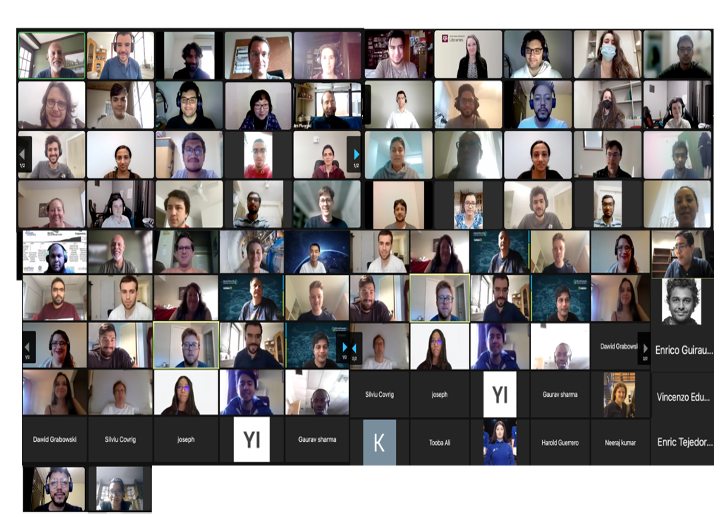
\includegraphics[width=0.90\textwidth]{images/software-carpentries-aug2021.png}
\end{figure}
\end{textblock}
\end{block}
\end{textblock}

\begin{textblock}{19.0}(63,61)
\begin{block}{Matplotlib 2022}
\begin{textblock}{19.0}(63,63)
\begin{figure}[tbph]
\centering
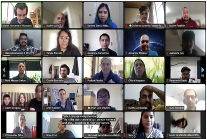
\includegraphics[width=1.00\textwidth]{images/matplotlib-2022-1.png}
\end{figure}
\end{textblock}
\end{block}
\end{textblock}


%%%%%%%%%%%%%%%%%%%%%%%%%%%%%%%%%%%%%%%%%%%%%%%%%%%%%%%%%%%%%%%%%%%%%%%%%%%%%%

\begin{textblock}{38.0}(2,61)
\begin{block}{HEP Software Foundation Training Center - Basic Curriculum}
\begin{textblock}{19.0}(2,63)
\begin{figure}[tbph]
\centering
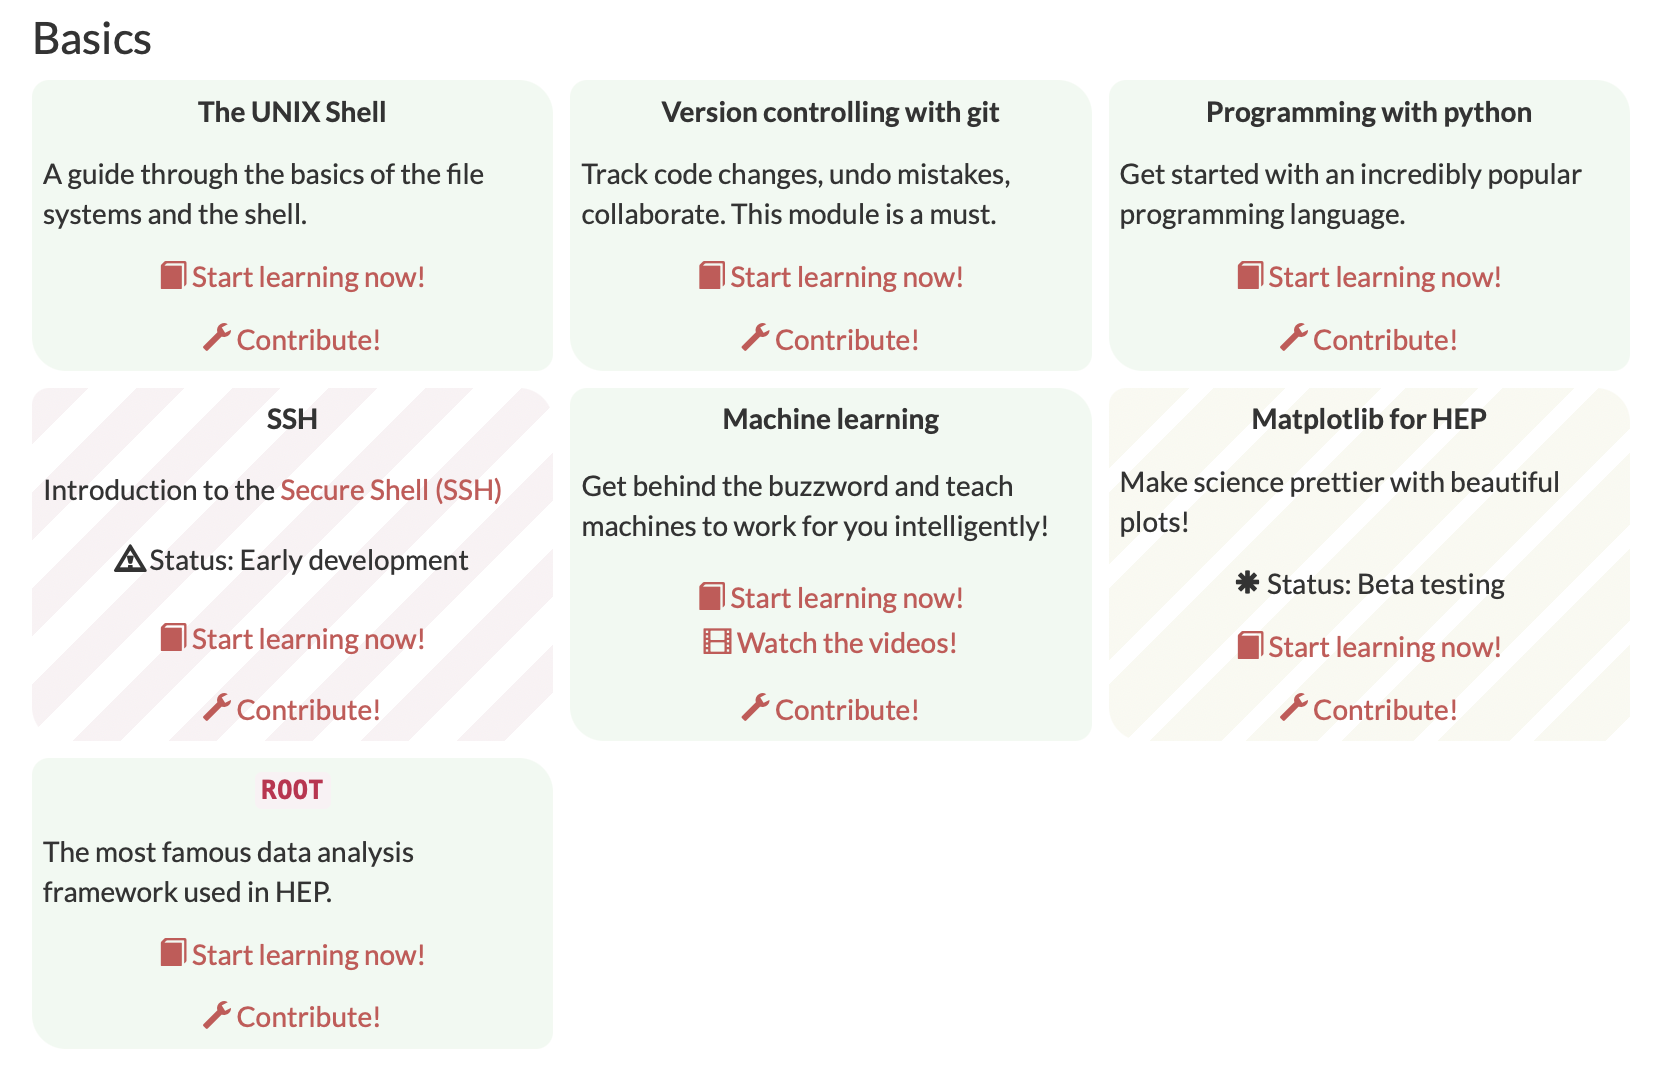
\includegraphics[width=1.00\textwidth]{images/hsf-training-1.png}
\end{figure}
\begin{figure}[tbph]
\centering
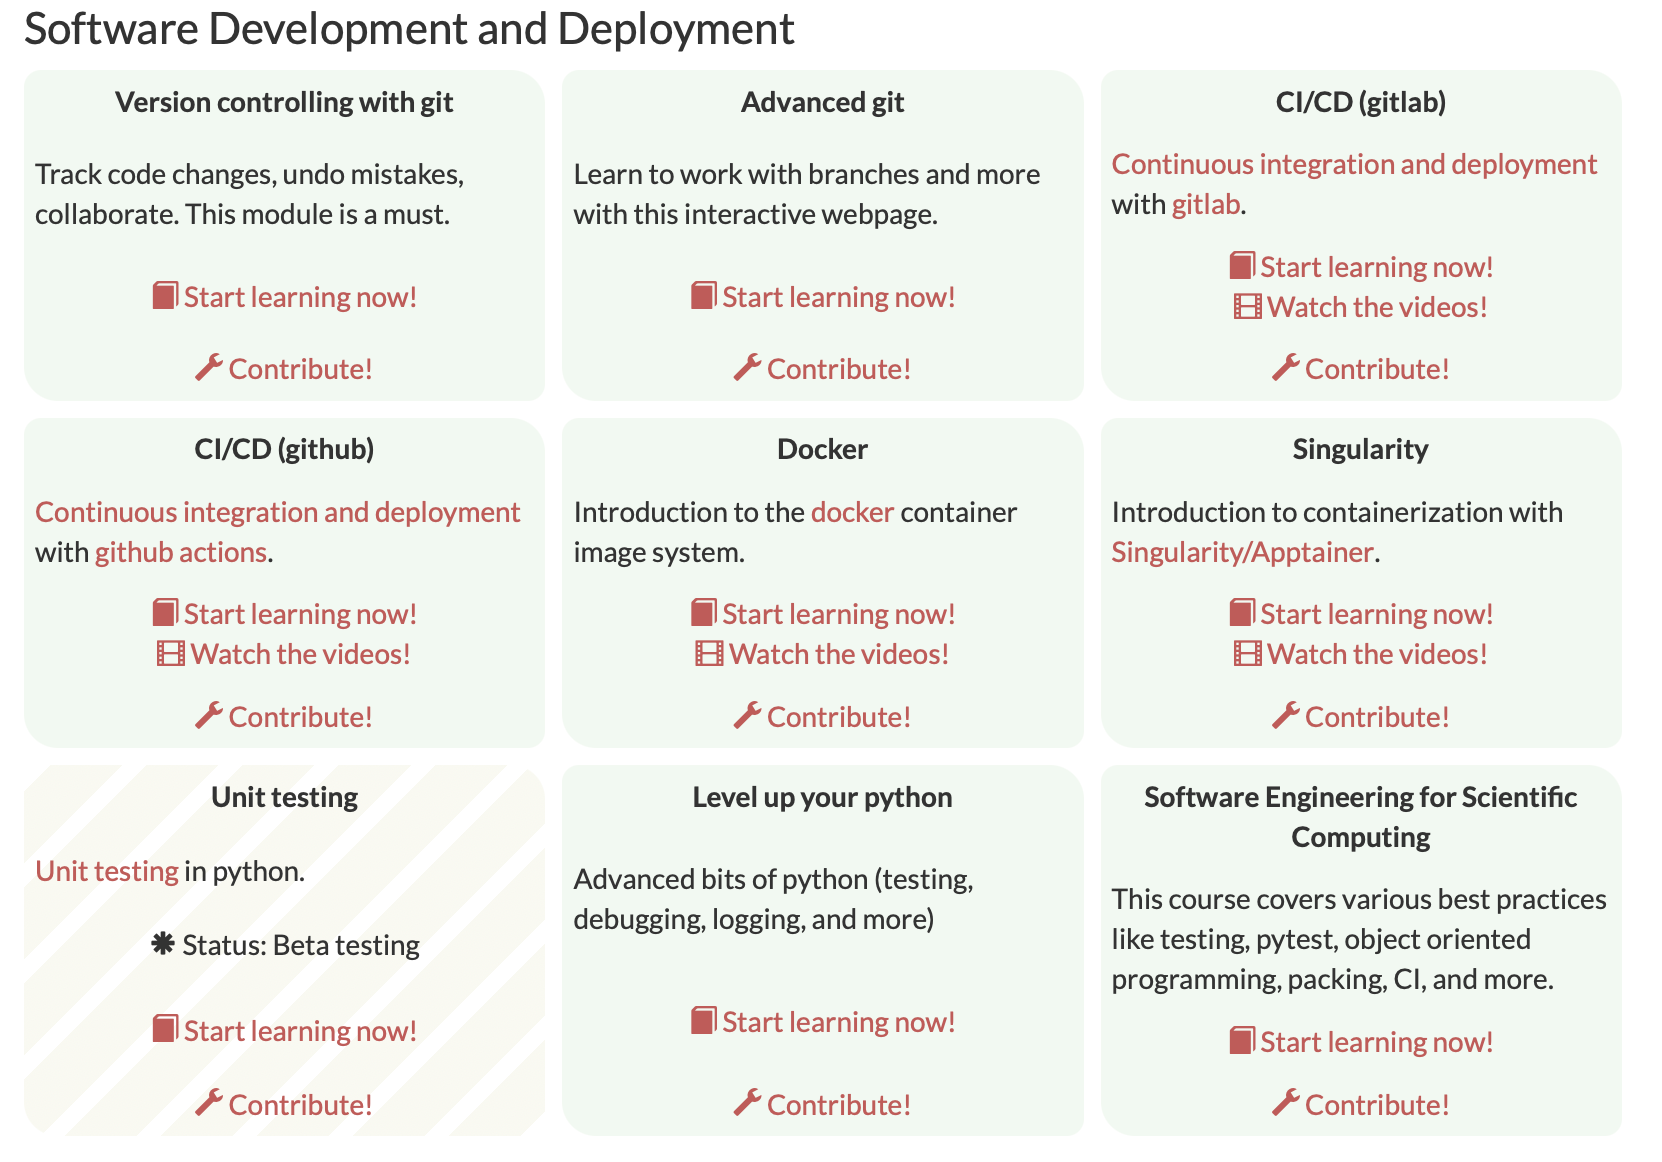
\includegraphics[width=1.00\textwidth]{images/hsf-training-2.png}
\end{figure}
\begin{figure}[tbph]
\centering
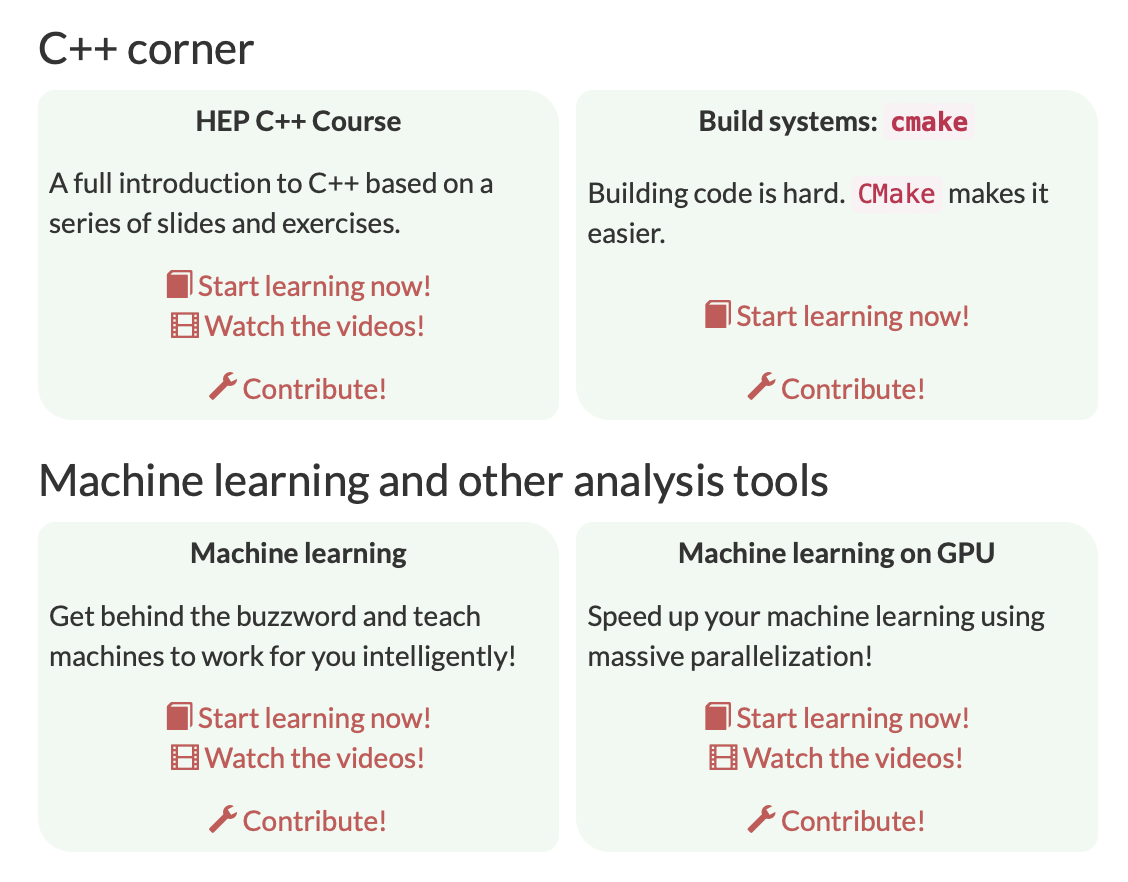
\includegraphics[width=1.00\textwidth]{images/hsf-training-3.png}
\end{figure}
\end{textblock}
\begin{textblock}{19.0}(21,63)
\begin{figure}[tbph]
\centering
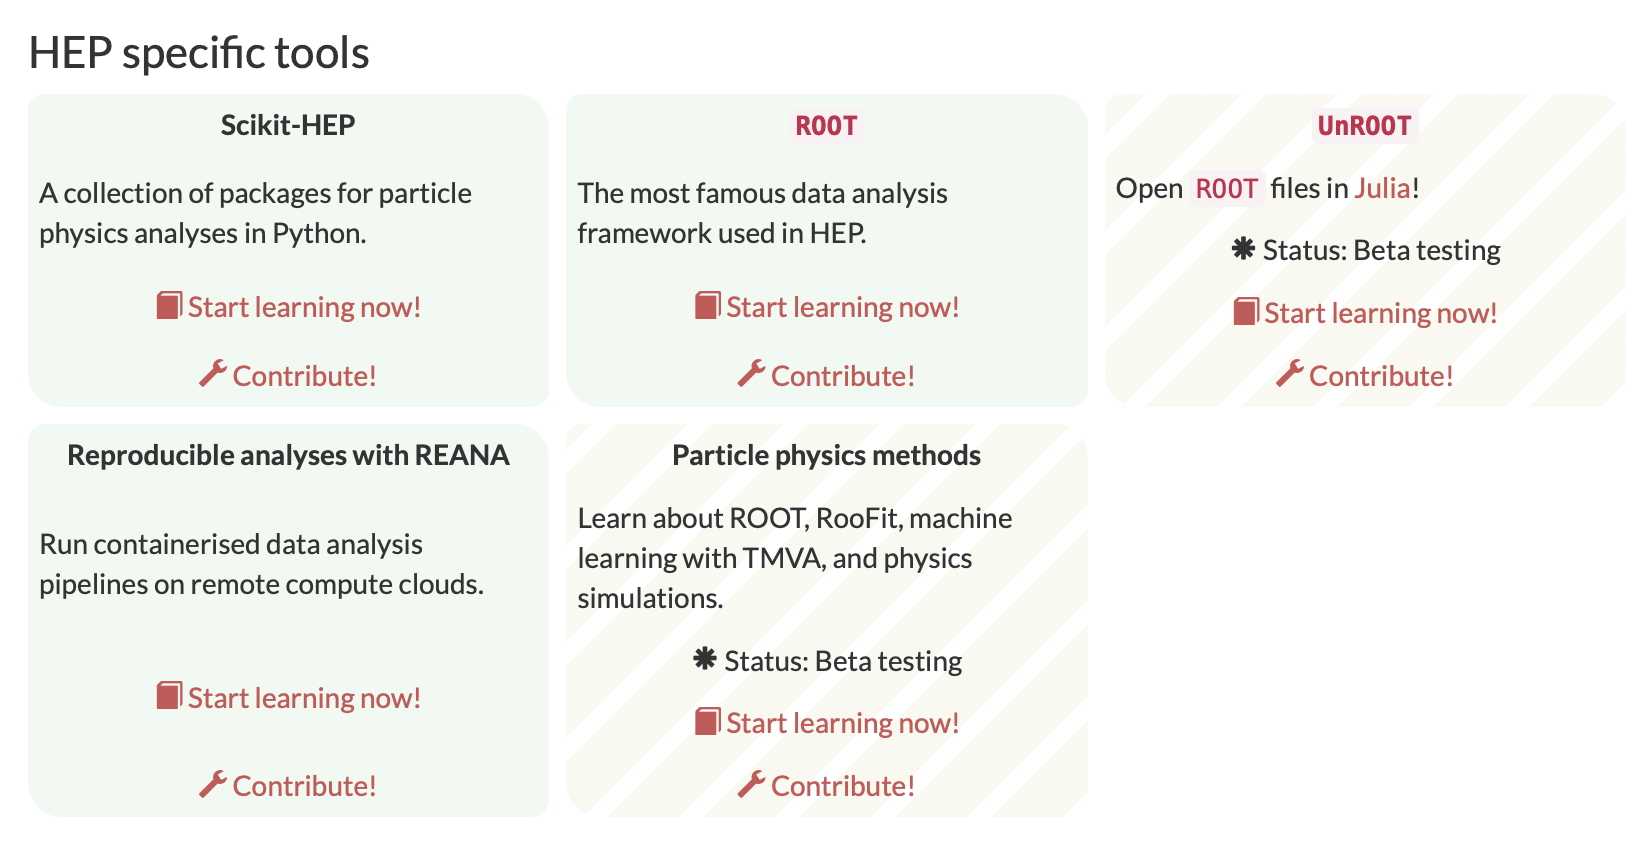
\includegraphics[width=1.00\textwidth]{images/hsf-training-4.png}
\end{figure}
\begin{figure}[tbph]
\centering
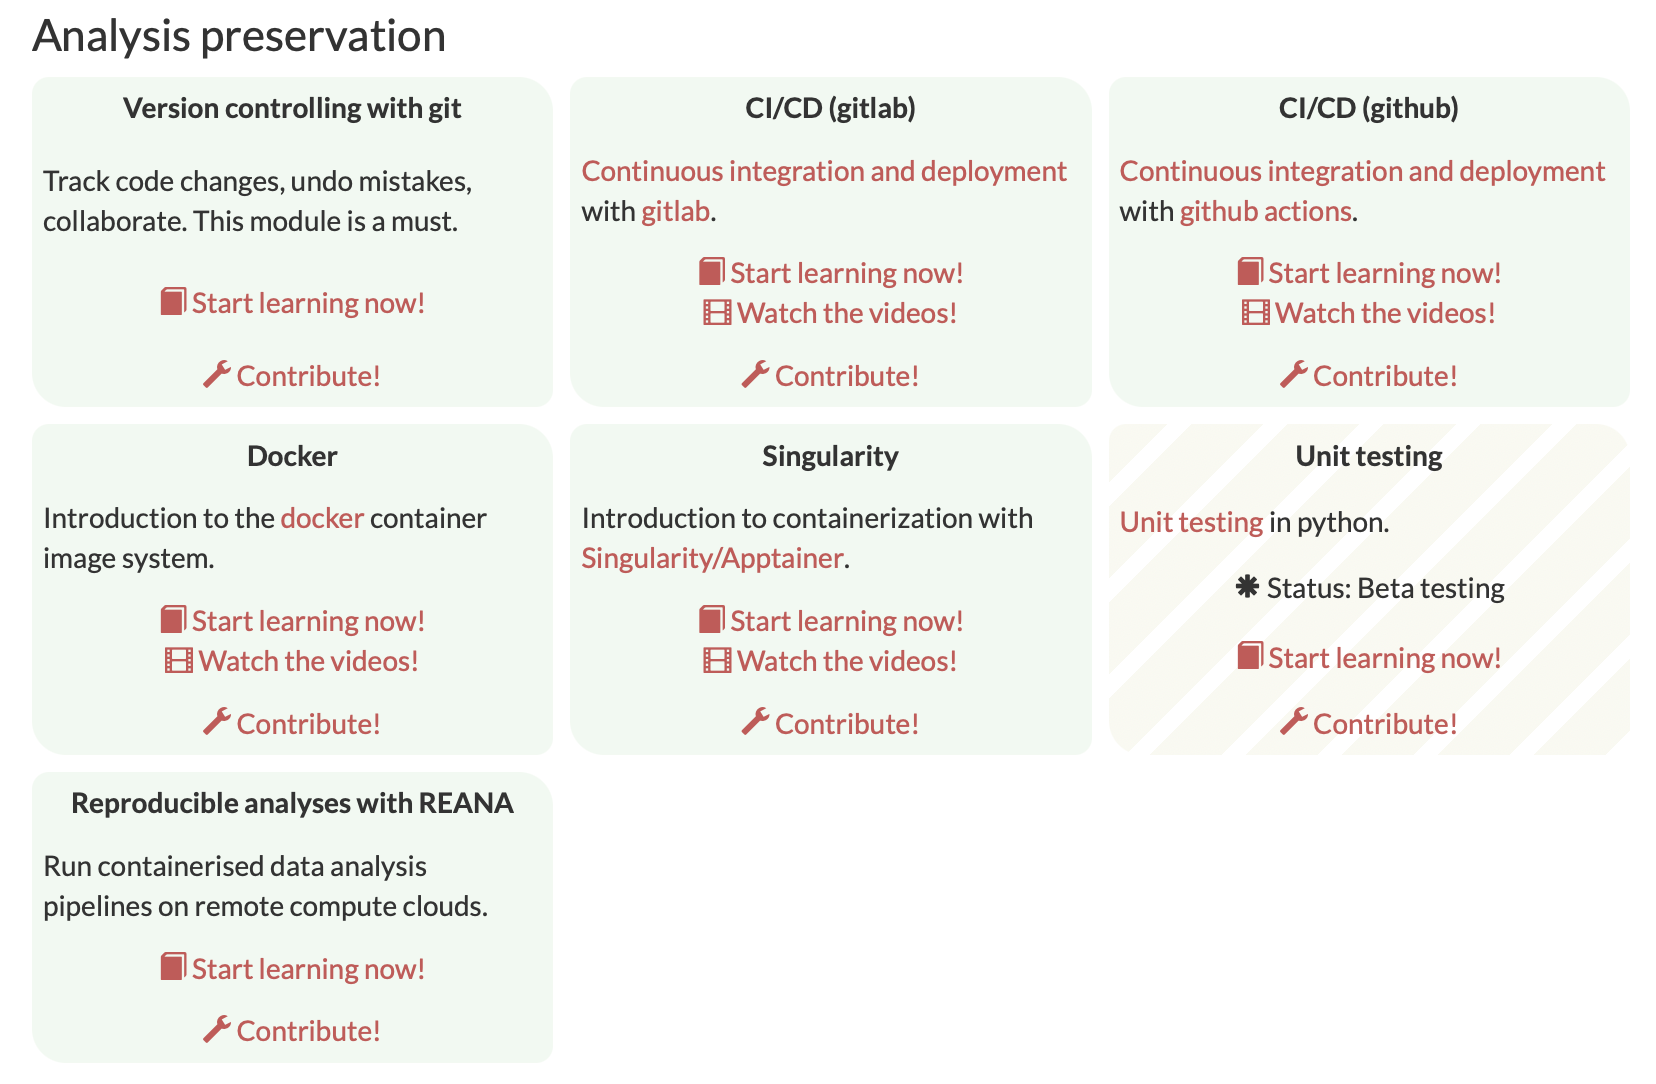
\includegraphics[width=1.00\textwidth]{images/hsf-training-5.png}
\end{figure}
\begin{figure}[tbph]
\centering
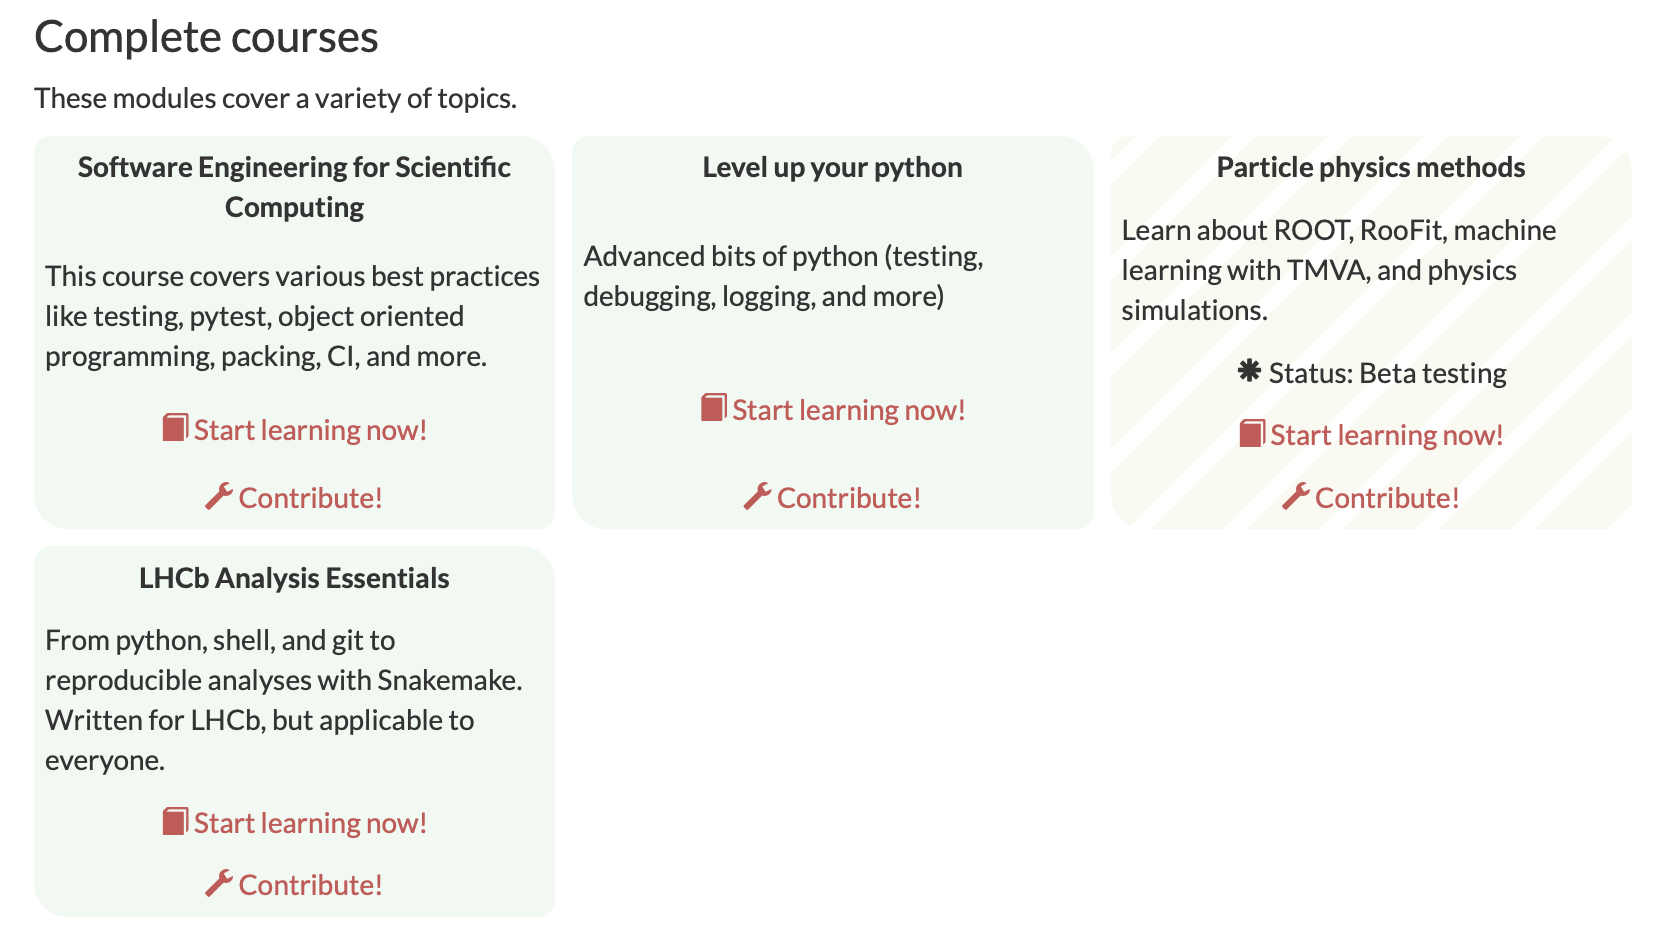
\includegraphics[width=1.00\textwidth]{images/hsf-training-6.png}
\end{figure}
\end{textblock}
\end{block}
\end{textblock}

%%%%%%%%%%%%%%%%%%%%%%%%%%%%%%%%%%%%%%%%%%%%%%%%%%%%%%%%%%%%%%%%%%%%%%%%%%%%%%


%%%%%%%%%%%%%%%%%%%%%%%%%%%%%%%%%%%%%%%%%%%%%%%%%%%%%%%%%%%%%%%%%%%%%%%%%%%%%%
\begin{textblock}{38.0}(44,76)
\begin{block}{CoDaS-HEP Summer School}
\begin{textblock}{38.0}(44,78)
\begin{figure}[tbph]
\centering
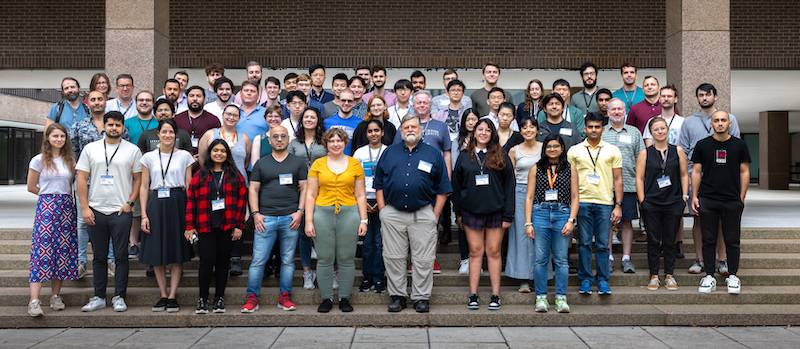
\includegraphics[width=1.00\textwidth]{images/codas-hep-2023-group-photo-thumbnail.jpg}
\end{figure}
The annual Computational and Data Science for HEP (CoDaS-HEP) summer school at Princeton provides more advanced training and helps build a larger ``cohort'' experience among graduate students and postdocs. The 5th school in July, 2023 involved more than 50 students and postdocs and a dozen lecturers. Topics covered include Parallel Programming, Advanced Data Science Tools and Techniques, Machine Learning - Technology and Methods and practical skills such as performance evaluation and collaborative use of git/github.
\end{textblock}
\end{block}
\end{textblock}
%%%%%%%%%%%%%%%%%%%%%%%%%%%%%%%%%%%%%%%%%%%%%%%%%%%%%%%%%%%%%%%%%%%%%%%%%%%%%%


\begin{textblock}{8.0}(4,107)
\begin{figure}[tbph]
\centering

\includegraphics[width=0.95\textwidth]{images/nsf1.jpg}
\end{figure}
\end{textblock}

\begin{textblock}{58.0}(12,108)
%\begin{block}{This poster online with links}
\begin{center}
This project is supported by National Science Foundation under grants OAC-1829707 and OAC-1829729. Any opinions, findings, conclusions or recommendations expressed in this material are those of the authors and do not necessarily reflect the views of the National Science Foundation.
%\end{block}
\end{center}
\begin{center}
\Large
\url{https://first-hep.org}
\end{center}

\end{textblock}

\begin{textblock}{8.0}(70,107)
%\begin{block}{This poster online with links}
\begin{figure}[tbph]
\centering

\includegraphics[width=0.95\textwidth]{images/nsf1.jpg}
\end{figure}
%\end{block}
\end{textblock}


\end{frame}
\end{document}
